In this subsection it is explained which microservices will be custom and which one will be used as pay-per-use. 
\\All microservices will be stored in the Cloud offered by IBM and every microservice is picked from the IBM Cloud Platform.
\\For services that are used with the pay-as-you-go mechanism it is briefly explained how they work and some diagrams are included to better understand the concept.
\begin{itemize}
	\item \textbf{Login - \href{https://cloud.ibm.com/catalog/services/app-id}{IBM App ID}}: \hypertarget{appidsafestreets}{This microservice} is about User Authentication and Management, and provides a log-in framework. App ID will be used to add authentication to our web and mobile apps securing our Cloud-native applications and services on IBM Cloud. By requiring users to sign in to our app, we will be able to store user data such as app preferences or information from public social profile to recognize user that reports violations and customize each user's experience within the app.
	\\When a user is successfully authenticated, the application receives tokens from App ID. The service uses three main types of tokens to complete the authentication process: Access Token, Identity Token and Refresh Token.
	\begin{figure}[h!]
		\makebox[\textwidth]{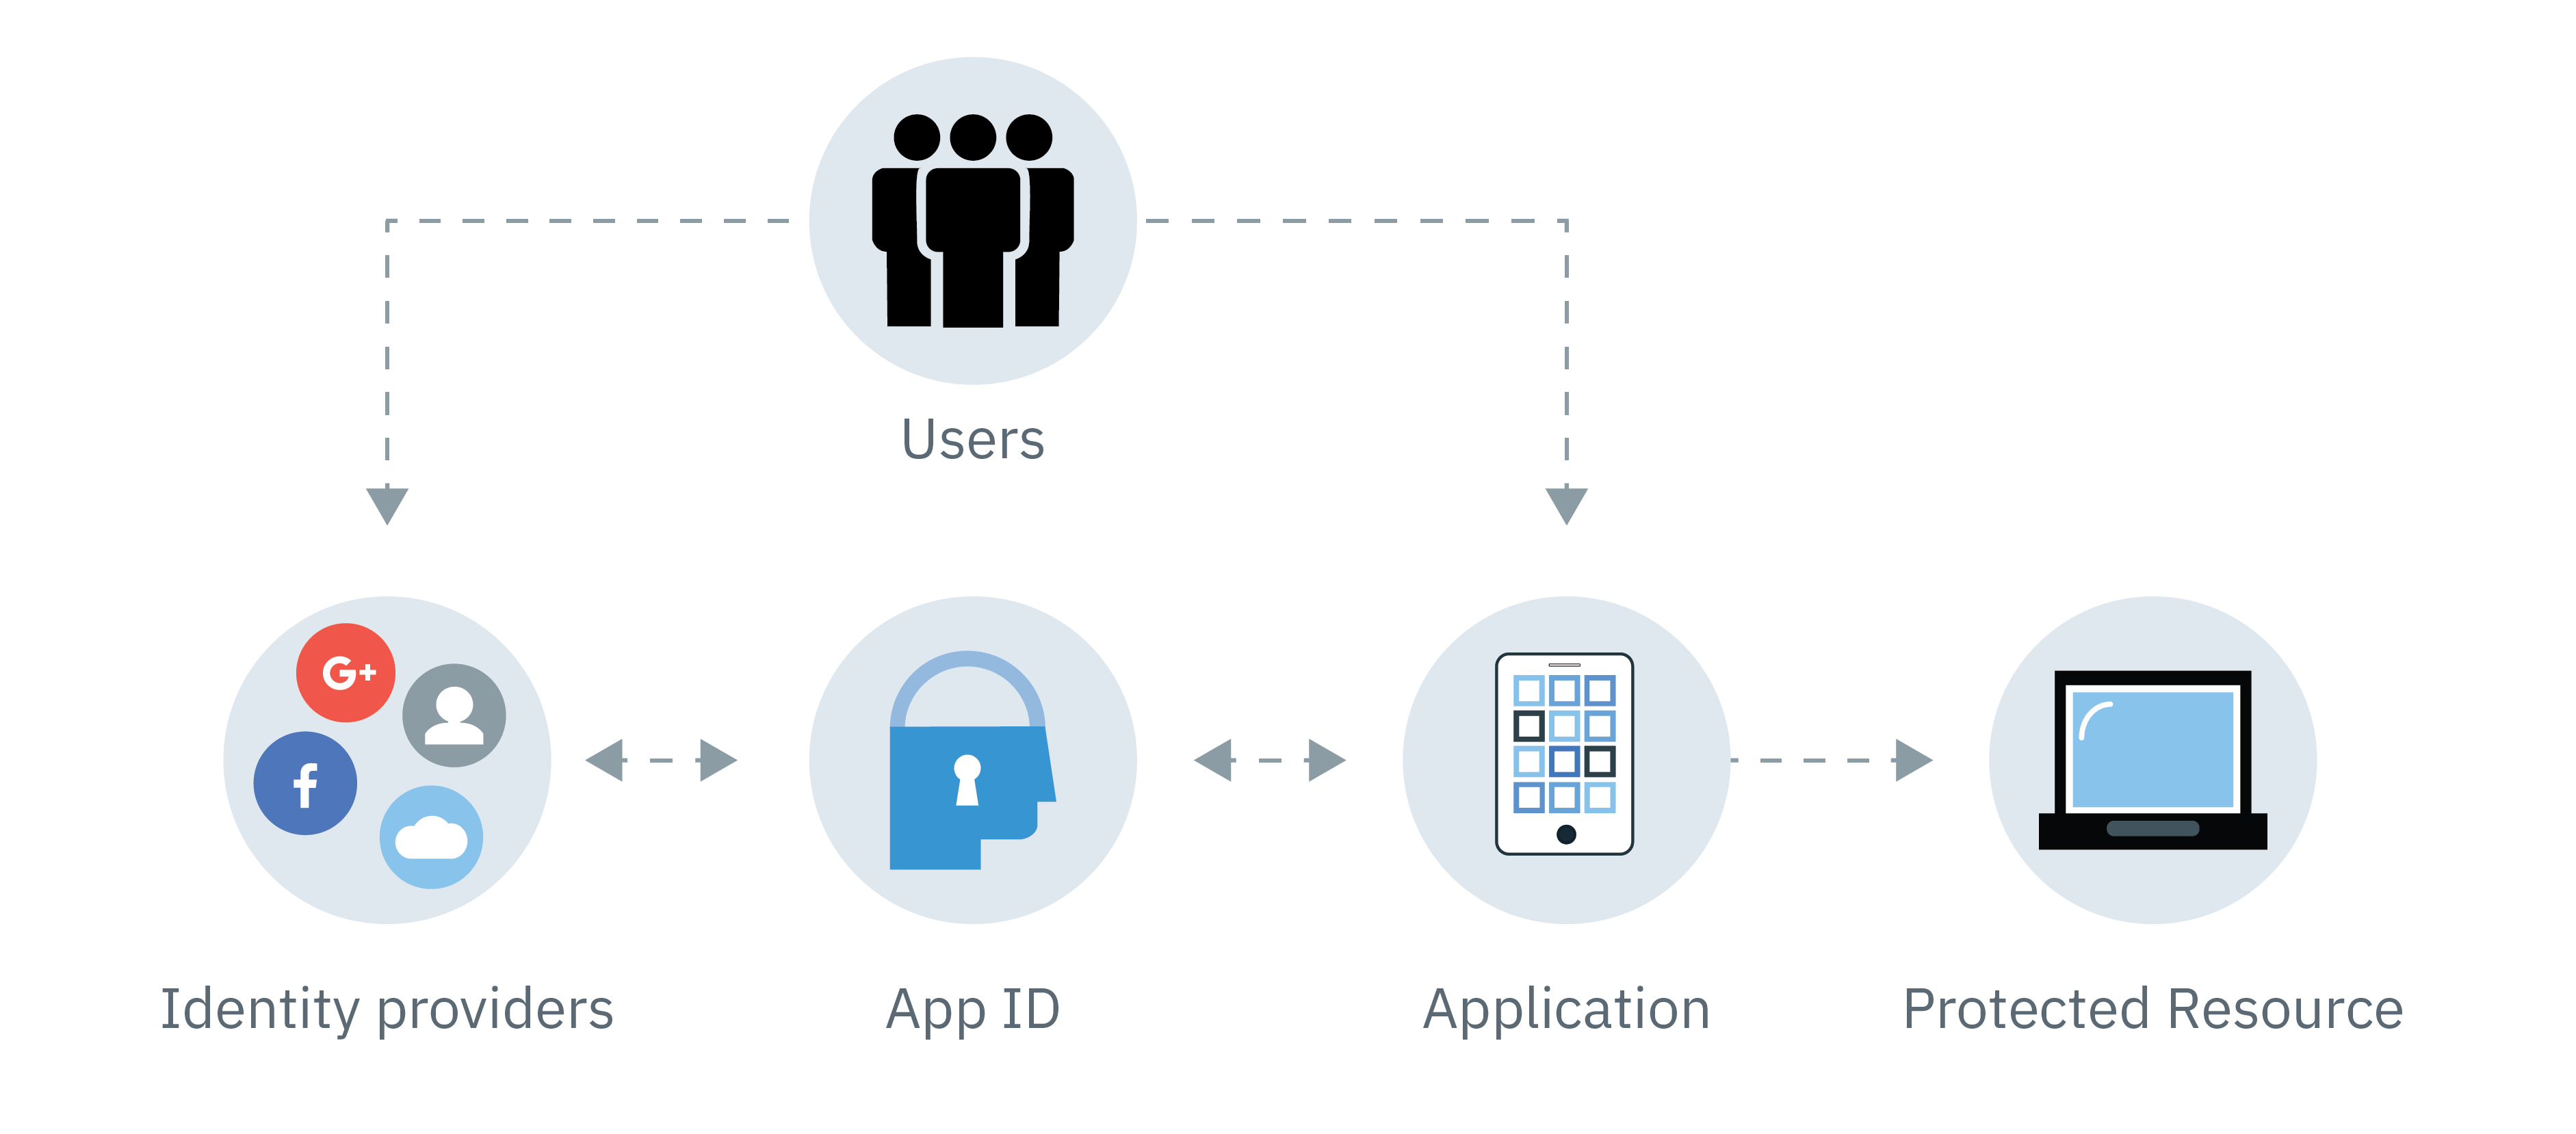
\includegraphics[width=1.15\textwidth]{/images/microservices/appidarchitecture.png}}
		\caption{IBM App ID working diagram.}
	\end{figure}
	\FloatBarrier

	\item \textbf{Computer Vision - \href{https://cloud.ibm.com/catalog/services/visual-recognition}{IBM Watson Visual Recognition}}: This service uses deep learning algorithms to analyze images for scenes, objects, and other content. In our scenario it will be used for certifying automatic tickets and to extract various information from violation's pictures.
	\\Its usage is simple as making an HTTP request to its POST API sending the image then wait for it to finish his work. The response that it returns includes keywords that provide information about the content along with an estimate probability of them being identified.
	\\In addition, IBM Watson Visual Recognition supports high availability with no single point of failure. Recovering from potential disasters that affect an entire IBM location requires planning and preparation but can always be done saving all of our custom training model.
	\begin{figure}[h!]
		\makebox[\textwidth]{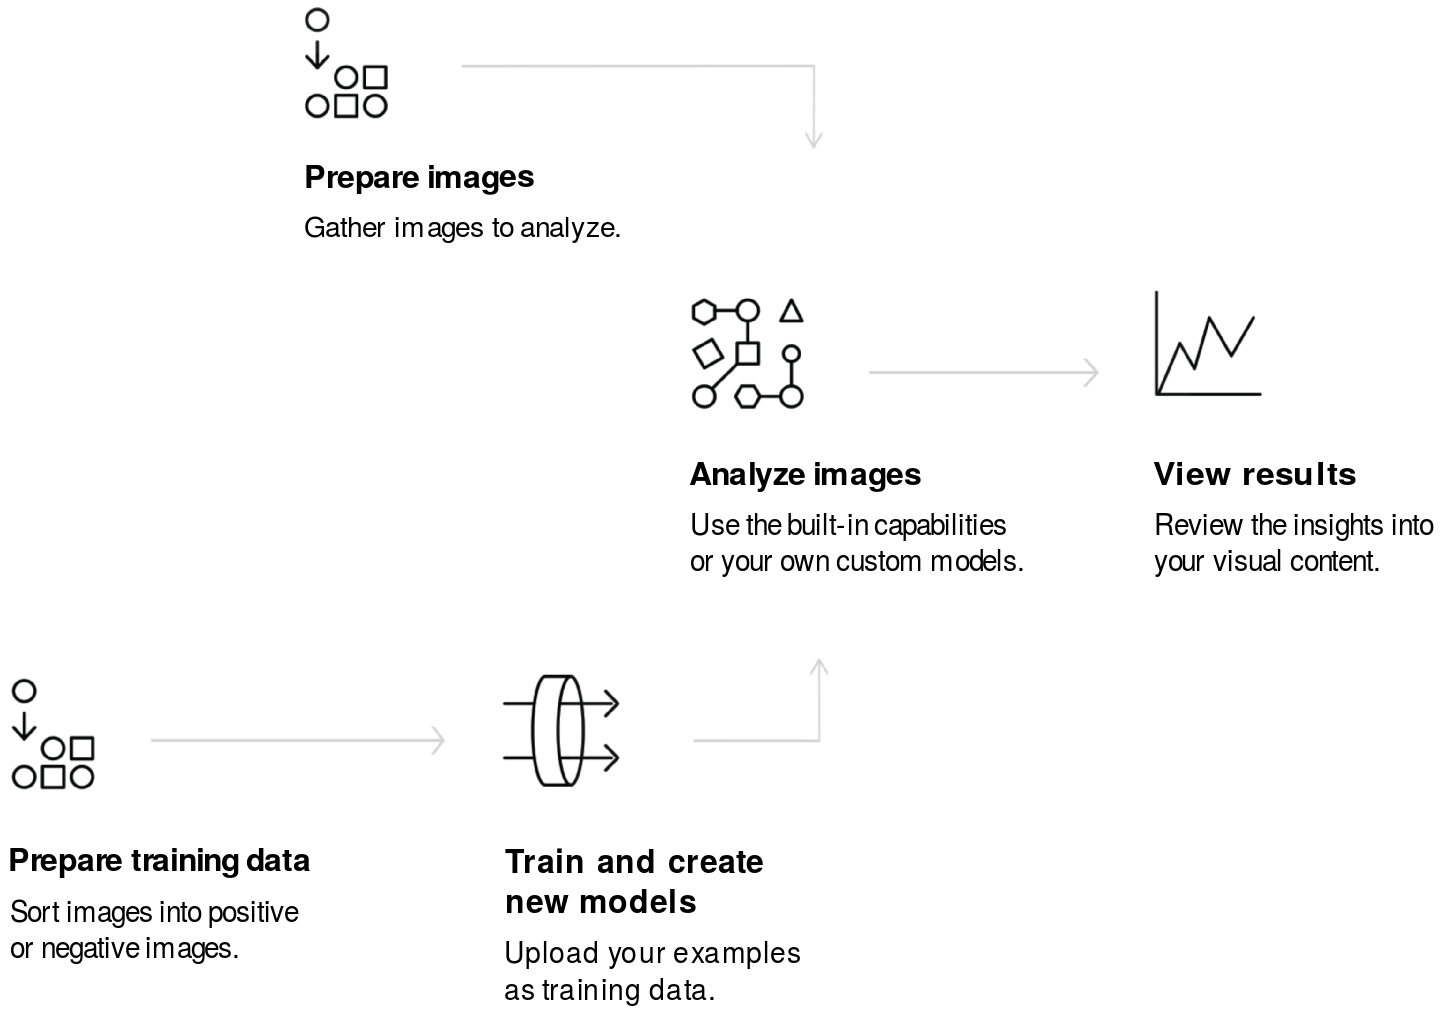
\includegraphics[width=1.15\textwidth]{/images/microservices/visualrecognition.png}}
		\caption{IBM Watson Visual Recognition working diagram.}
	\end{figure}
	\FloatBarrier
	
	\item \textbf{Data Mining - \href{https://cloud.ibm.com/catalog/services/discovery}{IBM Watson Discovery}}: IBM Watson Discovery makes it possible to rapidly build cognitive, cloud-based exploration applications that unlock insights hidden in unstructured data. 
	\\This microservice is particularly useful when, at a given time everyday, SafeStreets crosses data coming from the municipality with its own data to extract potential suggestions.
	\\With Discovery, it only takes a few steps to prepare our unstructured data coming from different sources and to create a query that will pinpoint the information SafeStreets needs. Discovery automatically uses data analysis combined with cognitive intuition to take the unstructured data and enriches it to discover hidden information.
	\begin{figure}[h!]
		\makebox[\textwidth]{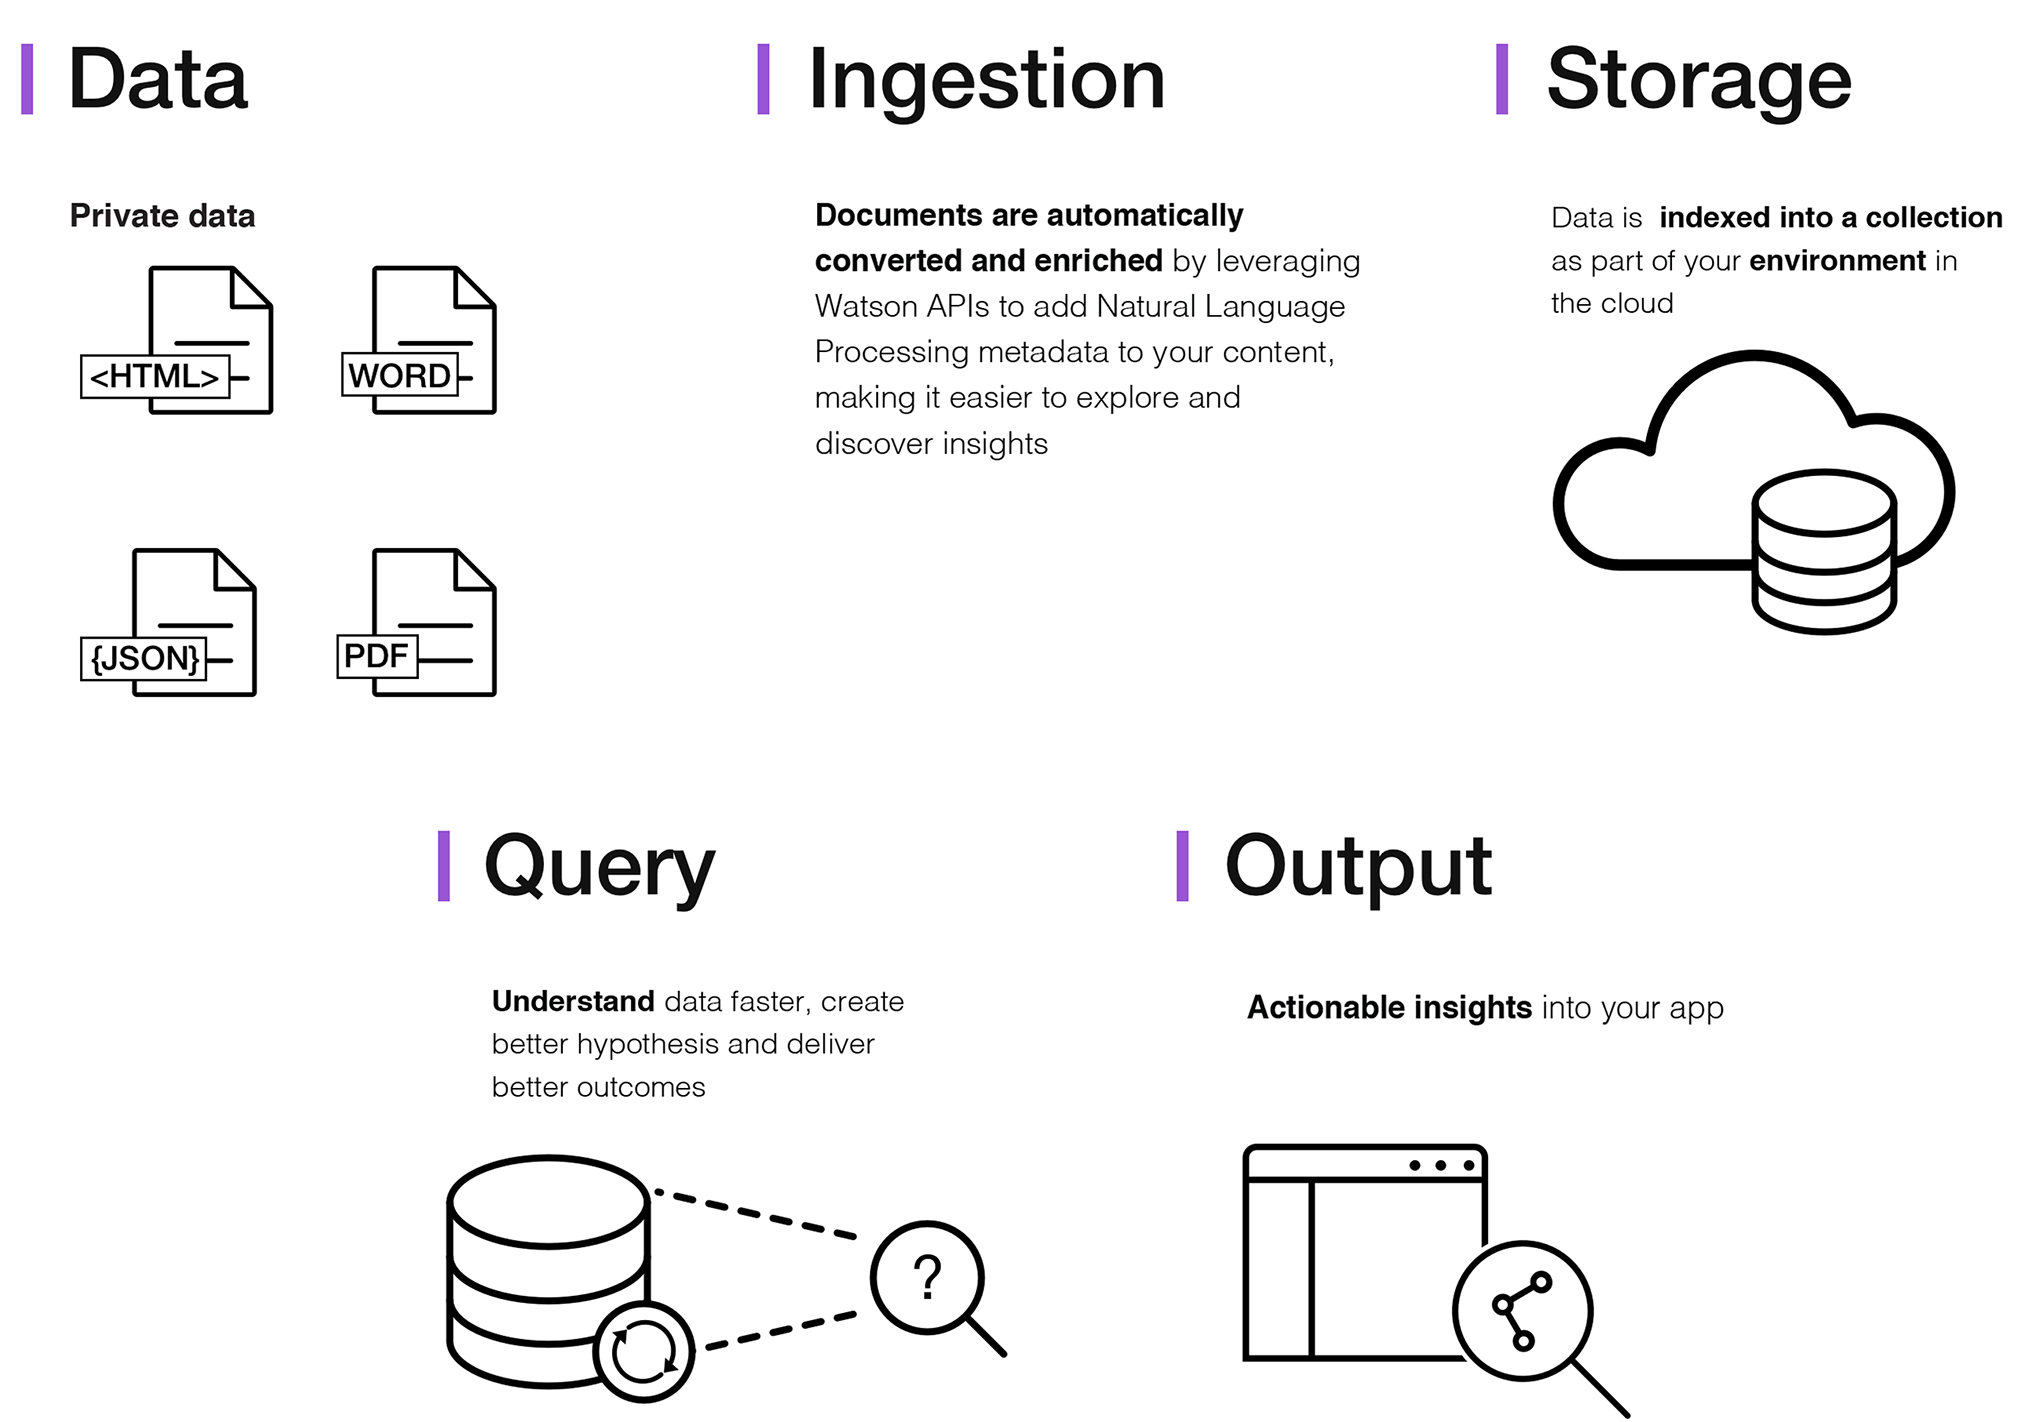
\includegraphics[width=1.25\textwidth]{/images/microservices/discoveryflow.png}}
		\caption{Complete architecture of our Discovery solution.}
	\end{figure}
	\FloatBarrier
	
	\item \textbf{Image Storage - \href{https://cloud.ibm.com/catalog/services/cloud-object-storage}{IBM Cloud Object Storage}}: When a user sends one or more pictures in a report along with various information on the violation he's reporting, these files must be obviously stored somewhere. In our case, to ensure  resiliency and the other proprieties expressed in the RASD, we opted for storing these image in the IBM Cloud. Indeed, information stored in the IBM Cloud Object Storage is encrypted and dispersed across multiple geographic locations, and accessed over HTTP using a modern RESTful API.
	In addition, IBM Cloud Object Storage allows SafeStreets to separate metadata from the image, but store them as objects in the same storage. That means that for every image, SafeStreets can associate it with highly unstructured data, different for each image. 
	\\For example when someone reports a violation, the related images are instantaneously saved in the Storage, along with their metadata. Then, when the Computer Vision algorithm takes place on them, the metadata of such images will be updated with a PUT request with the information that it will extract (such as the presence of no-parking signs).
	\\Last but not least, the IBM Cloud Object Storage can be easily associated with IBM Discovery as an external source for training.
	\begin{figure}[h!]
		\makebox[\textwidth]{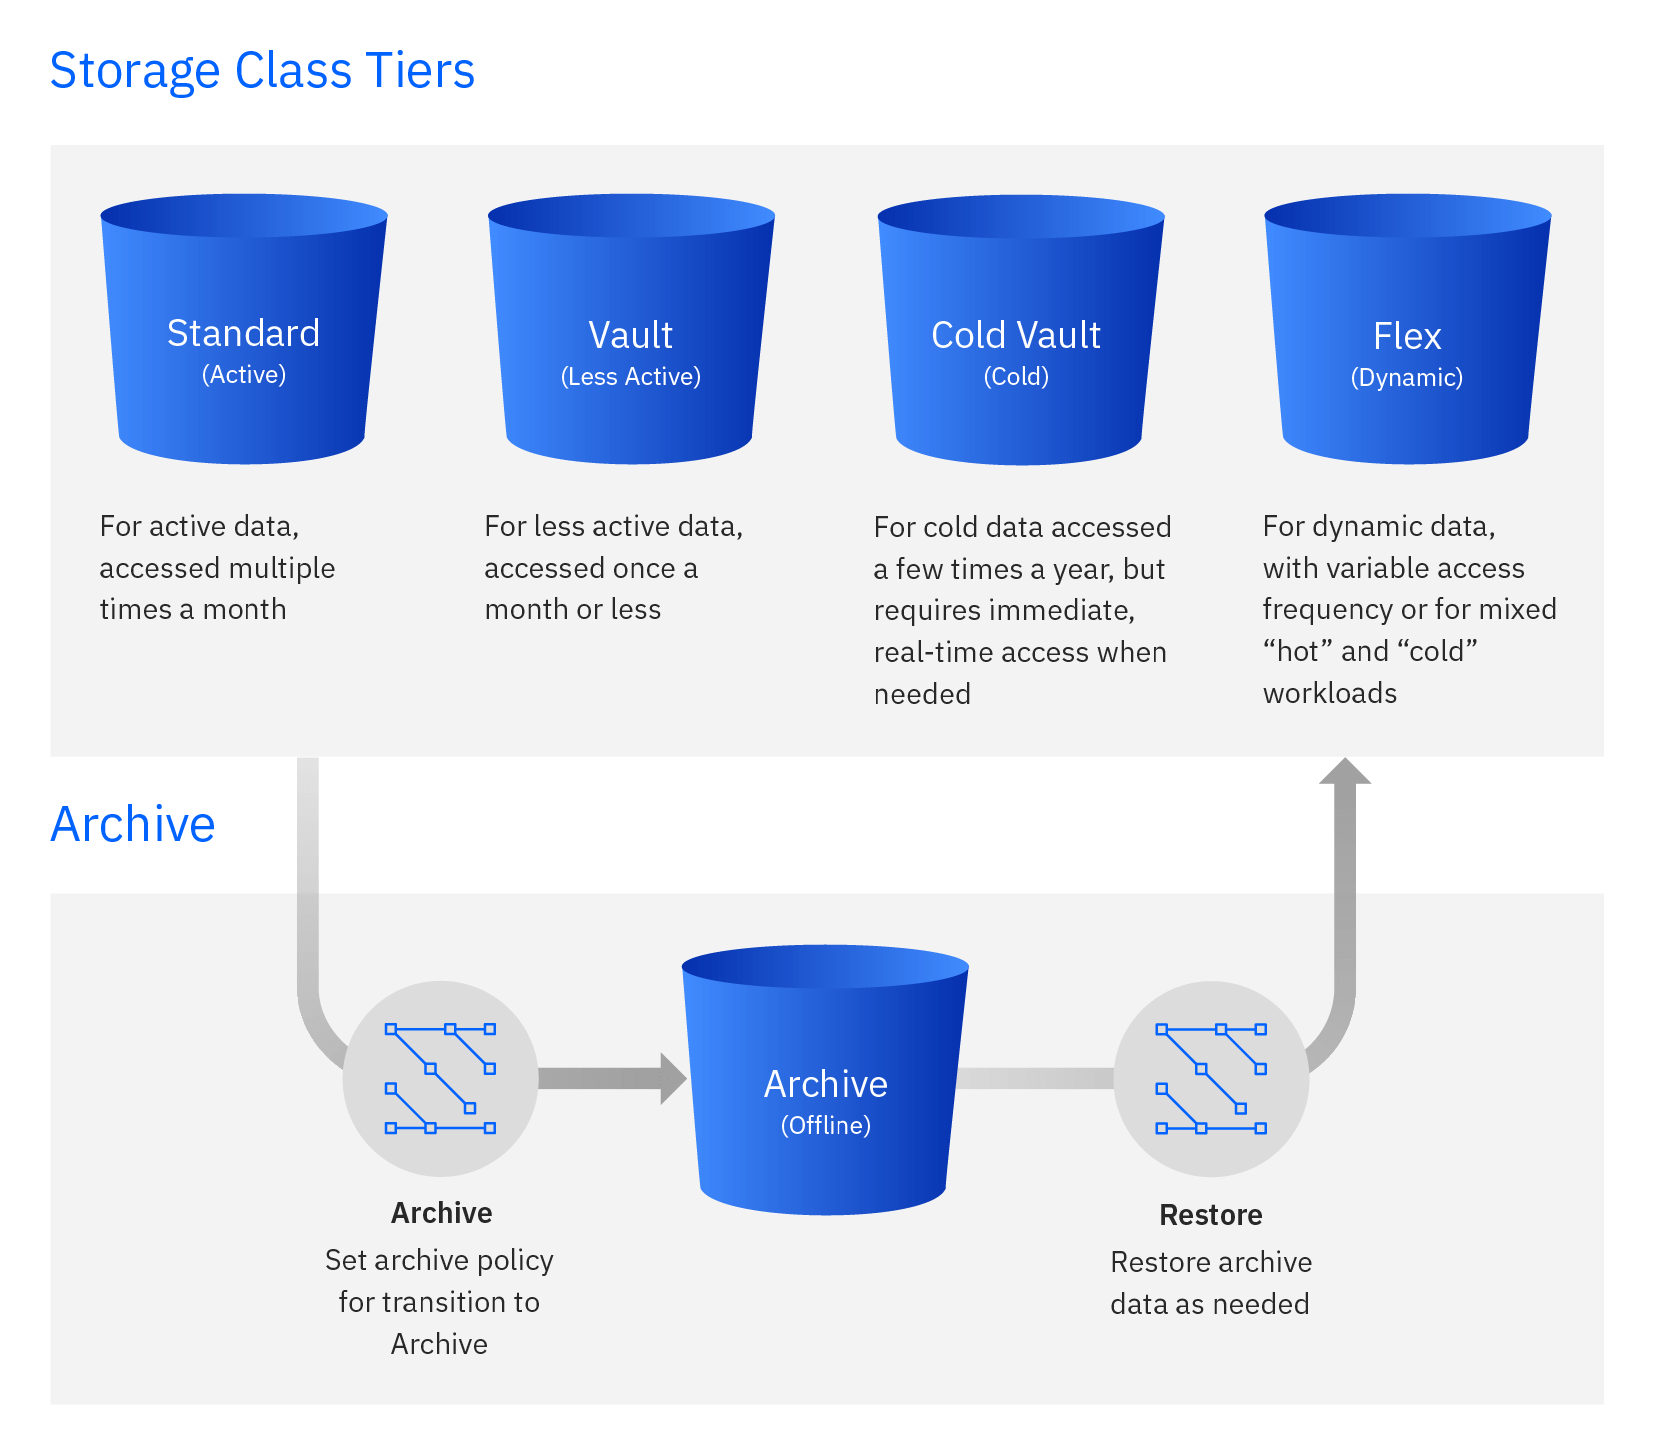
\includegraphics[width=0.95\textwidth]{/images/microservices/policybasedarchive.png}}
		\caption{IBM automatically tier data to the lowest-cost archive.}
	\end{figure}
	\FloatBarrier
	
	\item \textbf{NoSQL Database - \href{https://cloud.ibm.com/catalog/services/cloudant}{IBM Cloudant}}: IBM Cloudant is a distributed database that is optimized for handling heavy workloads that are typical of large, fast-growing web and mobile apps. Available as an SLA-backed, fully managed IBM Cloud service, Cloudant elastically scales throughput and storage independently.
	\\SafeStreets will use Cloudant every time a NoSQL Database is required, for example to manage the highly unstructured data in the Suggestion DB.
	Moreover, Cloudant is ISO27001, SOC 2.2 compliant and HIPAA ready. All data is encrypted over the wire and at rest. The service integrates with IBM Authentication and Management (IBM App ID) for granular access control at the API level.
	\\Using this service, SafeStreets will not need any server (Cloudant is serverless) and its data will be automatically replicated closer to all the places it needs to be, for uninterrupted data access.
	\begin{figure}[h!]
		\makebox[\textwidth]{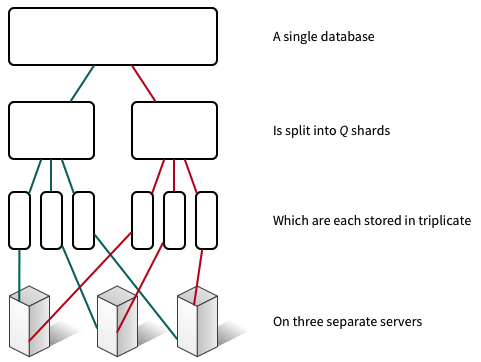
\includegraphics[width=0.9\textwidth]{/images/microservices/shardingdatabase.png}}
		\caption{How is data stored in IBM Cloudant}
	\end{figure}
	\FloatBarrier
	All Q shards together contain the data within database. Each shard is stored in three separate copies. Each shard copy is called a shard replica. Each shard replica is stored on a different server. The servers are available within a single location data center. The collection of servers in a data center is called a cluster.
	\begin{figure}[h!]
		\makebox[\textwidth]{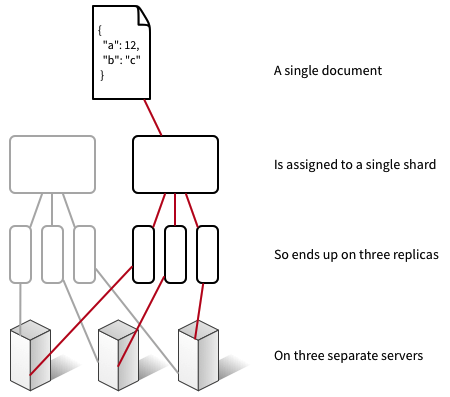
\includegraphics[width=0.9\textwidth]{/images/microservices/shardingdocument.png}}
		\caption{How is data stored in IBM Cloudant}
	\end{figure}
	\FloatBarrier
	
	\item \textbf{Relational Database - \href{https://cloud.ibm.com/catalog/services/databases-for-postgresql}{IBM Cloud Databases for PostgreSQL}}: A relational DBMS was chosen for all the Databases that contains structured data and on which many queries will be done (Violation, Statistics). Postgres was chosen over all database because it is a powerful, open source object-relational database with JSON support, that gives the best of both the SQL and NoSQL worlds. The advantages in using an IBM Cloud Service to deploy such service relies on the fact that this service allows us to scale disk and RAM independently to best fit SafeStreets application requirements.
	\\IBM Cloud Databases provide out-of-the-box integration with IBM Identity and Access Management that integrates completely into the SafeStreets architecture. 
	\begin{figure}[h!]
		\makebox[\textwidth]{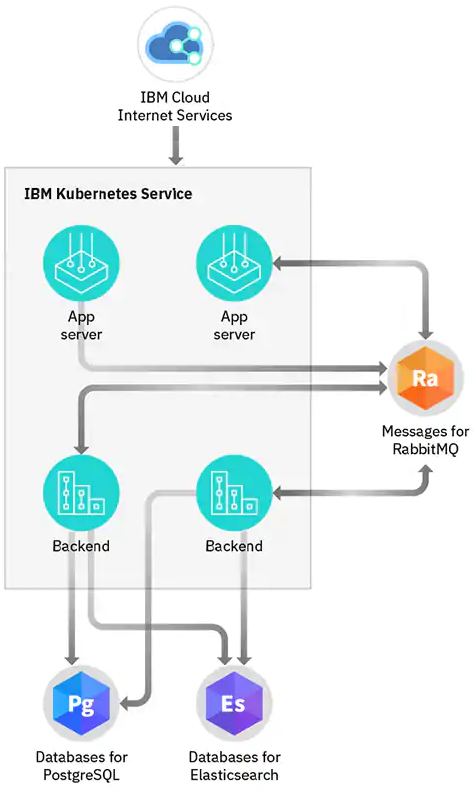
\includegraphics[width=0.7\textwidth]{/images/microservices/postgres.png}}
		\caption{Scalable SafeStreets architecture to handle millions of users.}
	\end{figure}
	\FloatBarrier
	
\end{itemize}